% Options for packages loaded elsewhere
\PassOptionsToPackage{unicode}{hyperref}
\PassOptionsToPackage{hyphens}{url}
\PassOptionsToPackage{dvipsnames,svgnames*,x11names*}{xcolor}
%
\documentclass[
]{article}
\usepackage{lmodern}
\usepackage{amsmath}
\usepackage{ifxetex,ifluatex}
\ifnum 0\ifxetex 1\fi\ifluatex 1\fi=0 % if pdftex
  \usepackage[T1]{fontenc}
  \usepackage[utf8]{inputenc}
  \usepackage{textcomp} % provide euro and other symbols
  \usepackage{amssymb}
\else % if luatex or xetex
  \usepackage{unicode-math}
  \defaultfontfeatures{Scale=MatchLowercase}
  \defaultfontfeatures[\rmfamily]{Ligatures=TeX,Scale=1}
\fi
% Use upquote if available, for straight quotes in verbatim environments
\IfFileExists{upquote.sty}{\usepackage{upquote}}{}
\IfFileExists{microtype.sty}{% use microtype if available
  \usepackage[]{microtype}
  \UseMicrotypeSet[protrusion]{basicmath} % disable protrusion for tt fonts
}{}
\makeatletter
\@ifundefined{KOMAClassName}{% if non-KOMA class
  \IfFileExists{parskip.sty}{%
    \usepackage{parskip}
  }{% else
    \setlength{\parindent}{0pt}
    \setlength{\parskip}{6pt plus 2pt minus 1pt}}
}{% if KOMA class
  \KOMAoptions{parskip=half}}
\makeatother
\usepackage{xcolor}
\IfFileExists{xurl.sty}{\usepackage{xurl}}{} % add URL line breaks if available
\IfFileExists{bookmark.sty}{\usepackage{bookmark}}{\usepackage{hyperref}}
\hypersetup{
  pdftitle={La Aveja Asiatica en Bizkaia 2018-2019},
  pdfauthor={Óscar Rojo Martín},
  colorlinks=true,
  linkcolor=Maroon,
  filecolor=Maroon,
  citecolor=Blue,
  urlcolor=blue,
  pdfcreator={LaTeX via pandoc}}
\urlstyle{same} % disable monospaced font for URLs
\usepackage[margin=1in]{geometry}
\usepackage{graphicx}
\makeatletter
\def\maxwidth{\ifdim\Gin@nat@width>\linewidth\linewidth\else\Gin@nat@width\fi}
\def\maxheight{\ifdim\Gin@nat@height>\textheight\textheight\else\Gin@nat@height\fi}
\makeatother
% Scale images if necessary, so that they will not overflow the page
% margins by default, and it is still possible to overwrite the defaults
% using explicit options in \includegraphics[width, height, ...]{}
\setkeys{Gin}{width=\maxwidth,height=\maxheight,keepaspectratio}
% Set default figure placement to htbp
\makeatletter
\def\fps@figure{htbp}
\makeatother
\setlength{\emergencystretch}{3em} % prevent overfull lines
\providecommand{\tightlist}{%
  \setlength{\itemsep}{0pt}\setlength{\parskip}{0pt}}
\setcounter{secnumdepth}{-\maxdimen} % remove section numbering
\usepackage{fancyhdr}
\usepackage{graphicx}
\pagestyle{fancy}
\setlength{\headheight}{12.69003pt}
\fancyfoot[L]{
\includegraphics[width=4cm]{footer.png}}
\fancyfoot[C]{Oscar Rojo Martín}
\fancyfoot[R]{\thepage}
\ifluatex
  \usepackage{selnolig}  % disable illegal ligatures
\fi

\title{La Aveja Asiatica en Bizkaia 2018-2019}
\author{Óscar Rojo Martín}
\date{Junio 2021}

\begin{document}
\maketitle

\renewcommand*\contentsname{Índice}
{
\hypersetup{linkcolor=}
\setcounter{tocdepth}{5}
\tableofcontents
}
\newpage

\pagebreak

\#La Avispa Asiatica en Bizkaia 2018-2019

\hypertarget{tuxedtulo-de-la-visualizaciuxf3n-donde-se-presentan-la-visualizaciuxf3n-realizada.-url-de-la-visualizaciuxf3n-y-del-cuxf3digo.-y-descripciuxf3n-corta-del-documento-y-del-que-se-presenta}{%
\subsubsection{1) Título de la visualización donde se presentan la
visualización realizada. URL de la visualización y del código. Y
descripción corta del documento y del que se
presenta}\label{tuxedtulo-de-la-visualizaciuxf3n-donde-se-presentan-la-visualizaciuxf3n-realizada.-url-de-la-visualizaciuxf3n-y-del-cuxf3digo.-y-descripciuxf3n-corta-del-documento-y-del-que-se-presenta}}

Presentación

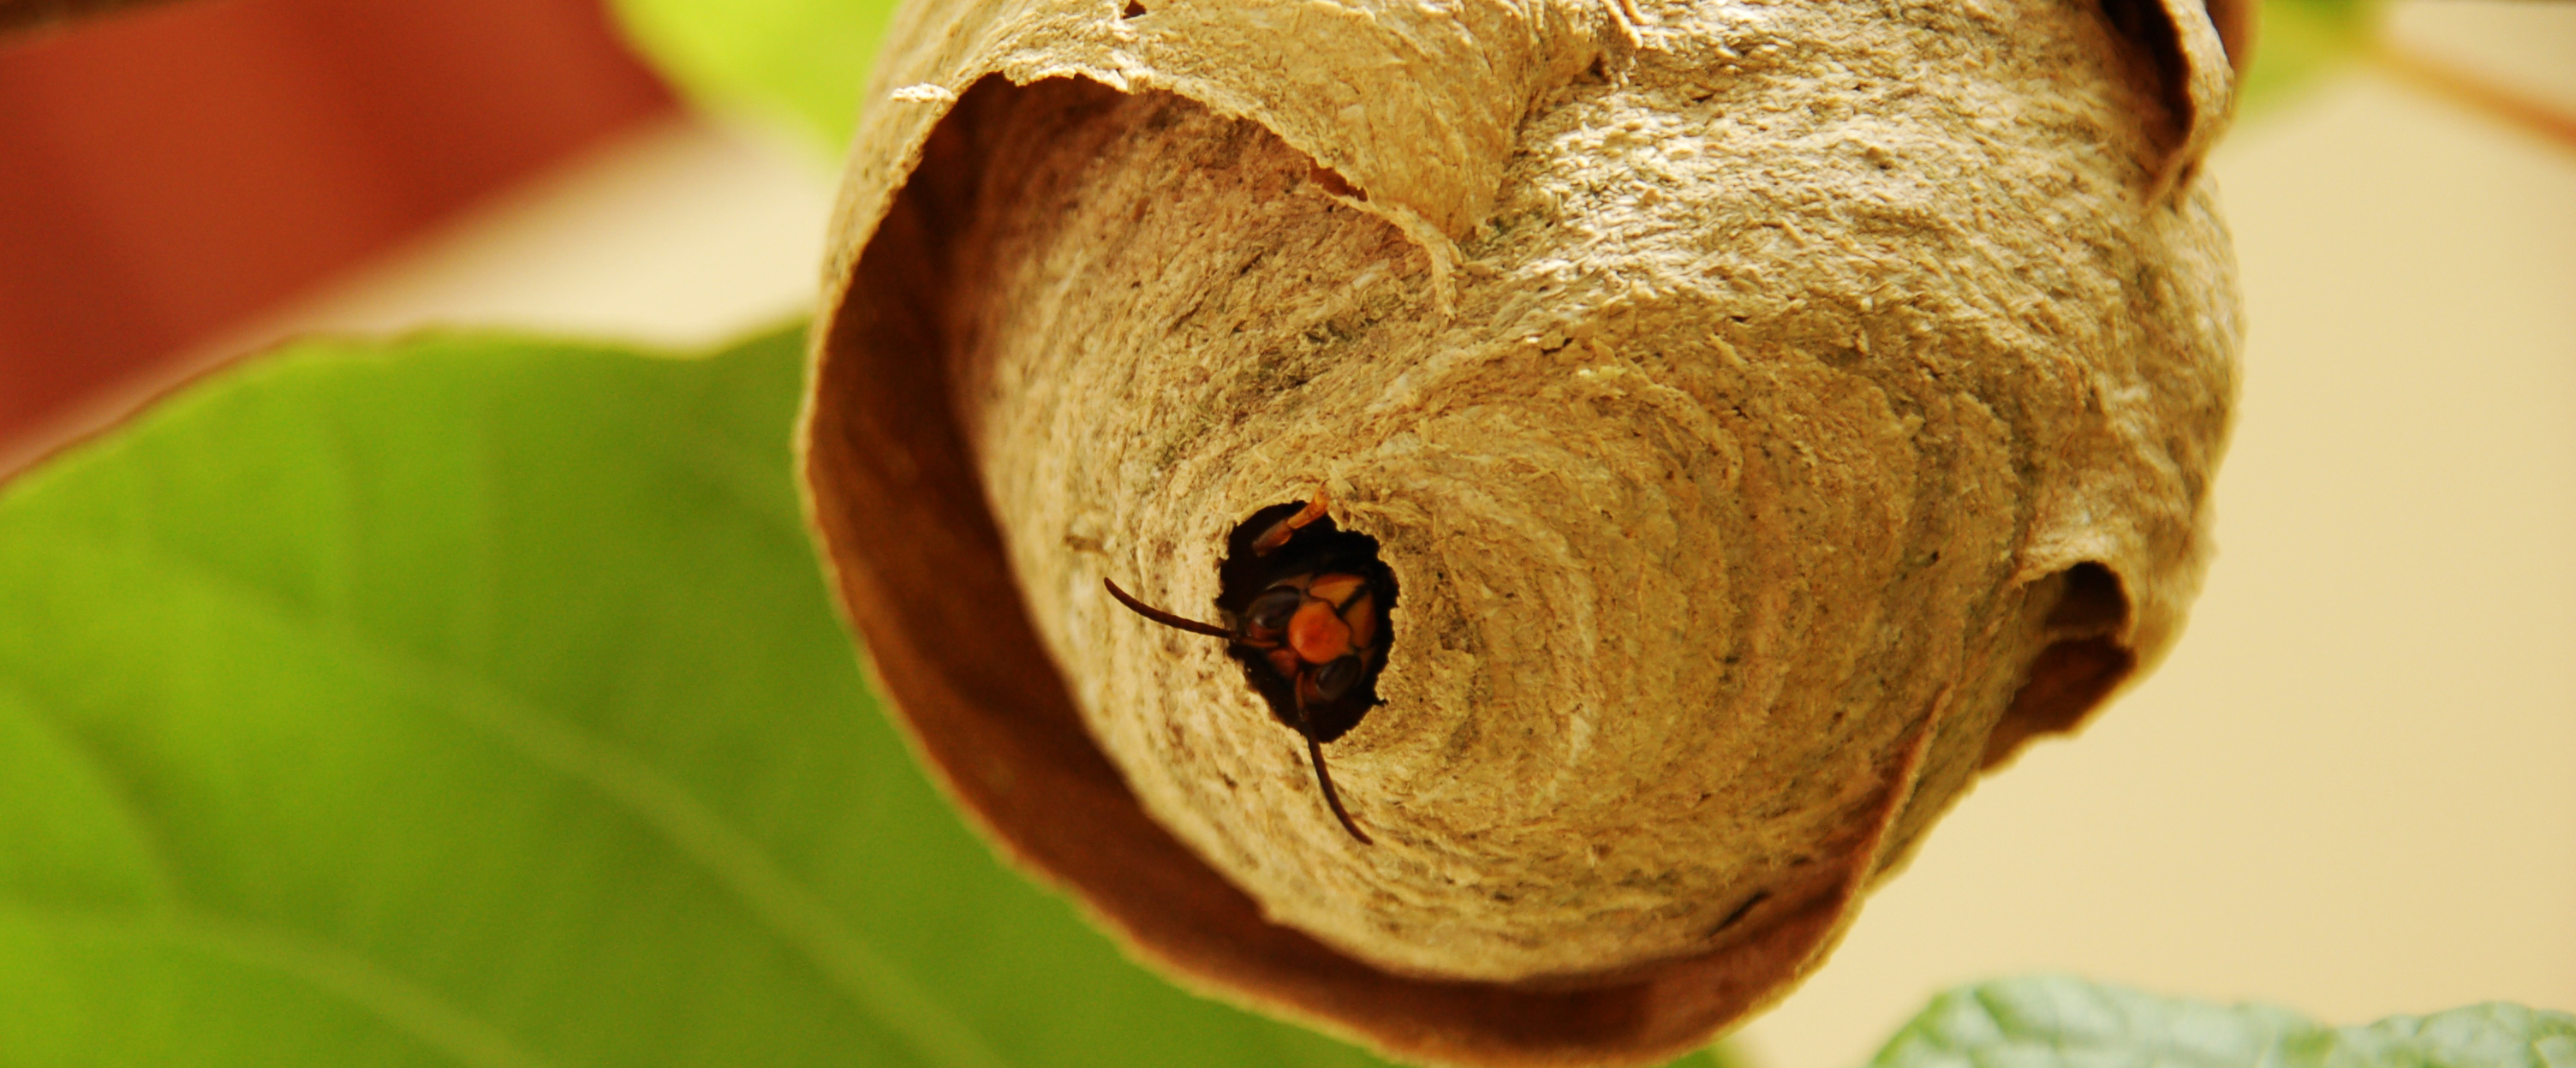
\includegraphics{Vespa/www/banner_vespas.jpg}

\hypertarget{un-tuxedtulo-que-sea-autoexplicativo-descriptivo.-que-contenga-palabras-clave.-que-atraiga-la-atenciuxf3n-de-los-lectores.}{%
\paragraph{1.1- Un título que sea autoexplicativo / descriptivo. Que
contenga palabras clave. Que atraiga la atención de los
lectores.}\label{un-tuxedtulo-que-sea-autoexplicativo-descriptivo.-que-contenga-palabras-clave.-que-atraiga-la-atenciuxf3n-de-los-lectores.}}

\begin{verbatim}
    La Avispa Asiatica en Bizkaia 2018-2019  
\end{verbatim}

\hypertarget{la-url-funciona-y-es-puxfablicamente-accesible.}{%
\paragraph{1.2- La URL funciona y es públicamente
accesible.}\label{la-url-funciona-y-es-puxfablicamente-accesible.}}

\url{https://zumaiauoc.github.io/vespa/}

\hypertarget{la-descripciuxf3n-es-cuidadosa-consistente-y-ayuda-a-presentar-la-visualizaciuxf3n.}{%
\paragraph{1.3 - La descripción es cuidadosa, consistente y ayuda a
presentar la
visualización.}\label{la-descripciuxf3n-es-cuidadosa-consistente-y-ayuda-a-presentar-la-visualizaciuxf3n.}}

\#\#\href{https://github.com/zumaiaUOC/vespa/blob/main/index.md}{Descripción}

\pagebreak

\hypertarget{explicar-razonadamente-quuxe9-preguntas-responde-la-visualizaciuxf3n-presentada-y-quuxe9-uso-puede-tener-por-un-usuario-tipo.}{%
\subsubsection{2) Explicar razonadamente qué preguntas responde la
visualización presentada y qué uso puede tener por un usuario
tipo.}\label{explicar-razonadamente-quuxe9-preguntas-responde-la-visualizaciuxf3n-presentada-y-quuxe9-uso-puede-tener-por-un-usuario-tipo.}}

Explicación visualización

\hypertarget{quuxe9-visualizaciuxf3n-se-ha-escogido-por-quuxe9}{%
\paragraph{2.1- Qué visualización se ha escogido? Por
qué?}\label{quuxe9-visualizaciuxf3n-se-ha-escogido-por-quuxe9}}

Se han escogido varias visualizaciónes y en diferentes formatos.

Se ha realizado un Dashboard-Panel de control, con multiples filtros
para obtener el número de nidos por municipio entre otras cosas.

\href{https://oscar-rojo-martin.shinyapps.io/Vespa/}{
\includegraphics{img/datastudio.png}}

\url{https://oscar-rojo-martin.shinyapps.io/Vespa/}

\begin{center}\rule{0.5\linewidth}{0.5pt}\end{center}

Se ha generado un aplicación para mostrar en pantalla la ubicación de
los nidos detectados y posteriormente el detalle de los mismos en
formato tabla.

\href{https://oscar-rojo-martin.shinyapps.io/Vespa/}{
\includegraphics{img/shinyapp.png}}

\url{https://oscar-rojo-martin.shinyapps.io/Vespa/}

\begin{center}\rule{0.5\linewidth}{0.5pt}\end{center}

Por último se ha generado un archivo html con varias transformaciones y
visualizaciones de varios datasets

\href{https://rpubs.com/zumaia/vespa}{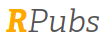
\includegraphics{img/rpubs.png}}

\url{https://rpubs.com/zumaia/vespa}

\hypertarget{para-quuxe9-y-para-quiuxe9n-puede-servir-esta-visualizaciuxf3n}{%
\paragraph{2.2- Para qué y para quién puede servir esta
visualización?}\label{para-quuxe9-y-para-quiuxe9n-puede-servir-esta-visualizaciuxf3n}}

Para toda persona interesada en la expansión de la Avispa Asiatica en
Bizkaia y para conocer muchos datos sobre ella.\\
En un futuro se podría predecir la evolución de la implantación de esta
especie invasora, etc\ldots{}

\pagebreak

\hypertarget{descripciuxf3n-tuxe9cnica-del-proyecto-lenguajes-libreruxedas-licencias-descripciuxf3n-tuxe9cnica-del-proyecto.}{%
\subsubsection{3) Descripción técnica del proyecto: lenguajes,
librerías, licencias, descripción técnica del
proyecto.}\label{descripciuxf3n-tuxe9cnica-del-proyecto-lenguajes-libreruxedas-licencias-descripciuxf3n-tuxe9cnica-del-proyecto.}}

Descripción Técnica del proyecto:

\hypertarget{quuxe9-transformaciuxf3n-de-datos-ha-habido-que-hacer-respecto-al-juego-de-datos-inicial}{%
\paragraph{3.1- Qué transformación de datos ha habido que hacer respecto
al juego de datos
inicial?}\label{quuxe9-transformaciuxf3n-de-datos-ha-habido-que-hacer-respecto-al-juego-de-datos-inicial}}

Se han realizado multiples transformaciones.

\href{https://rpubs.com/zumaia/vespa}{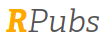
\includegraphics{img/rpubs.png}}

Se han integrado datasets, se ha realizado limpieza de datos, se ha
convertido datos en formato UTM a lat/lng. etc\ldots{}

\hypertarget{quuxe9-lenguaje-libreruxeda-software-has-usado-y-por-quuxe9}{%
\paragraph{3.2- Qué lenguaje, librería, software has usado y por
qué?}\label{quuxe9-lenguaje-libreruxeda-software-has-usado-y-por-quuxe9}}

El SO utilizado es Linux:\\
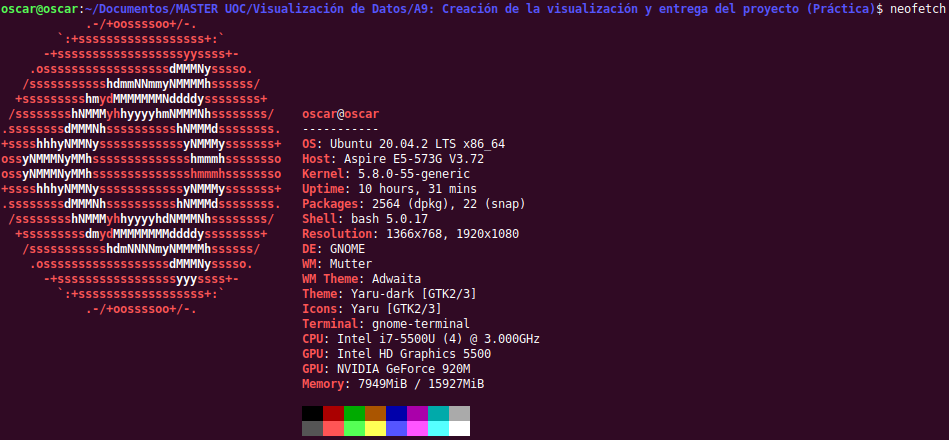
\includegraphics{img/linux.png}

Los Lenguajes de programación utilizados son:\\
- Python\\
- R\\
- HTML\\
- CSS

Los IDEs utilizados son:\\
- Pycharm\\
- Jupyter Lab\\
- RStudio

\pagebreak

\hypertarget{las-visualizaciones-realizadas}{%
\subsubsection{4) La/s visualizaciones
realizadas}\label{las-visualizaciones-realizadas}}

Visualización de datos.

\href{https://zumaiauoc.github.io/vespa/}{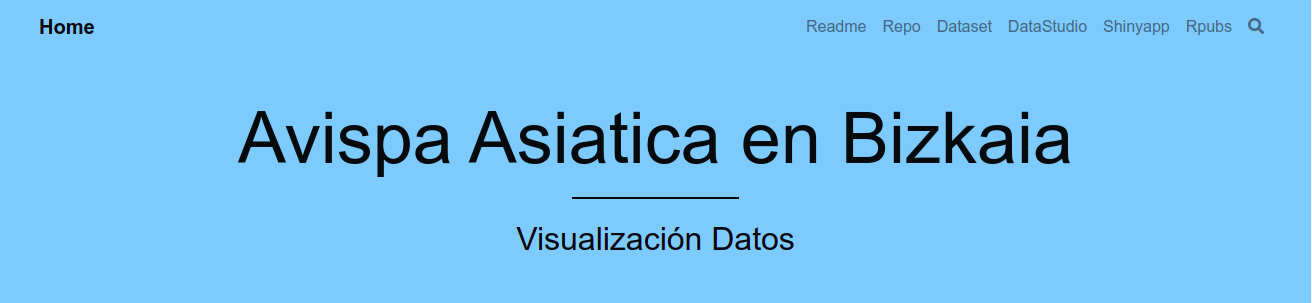
\includegraphics{img/vespa.png}}

El proyecto presentado cumple los siguientes bjetivos:

1- La visualización comunica bien los objetivos (título y layout).\\
2- La visualización responde las preguntas propuestas.\\
3- Interacciones presentes y con una justificación correcta.\\
4- Buena performance.\\
5- Diseño de color correcto.\\
6- Diseño de textos (títulos, leyendas\ldots) correctos.

\href{https://oscar-rojo-martin.shinyapps.io/Vespa/}{
\includegraphics{img/shinyapp.png}}\\
\href{https://oscar-rojo-martin.shinyapps.io/Vespa/}{
\includegraphics{img/datastudio.png}}\\
\href{https://rpubs.com/zumaia/vespa}{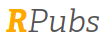
\includegraphics{img/rpubs.png}}

\pagebreak

\hypertarget{entrega-de-documentos.}{%
\subsubsection{5) Entrega de documentos.}\label{entrega-de-documentos.}}

Todos los documentos estan subidos a Github. Se subirá documento con las
URLs.

\end{document}
